\section{HIGH LEVEL SYSTEM ARCHITECTURE}
The system\textquotesingle s main components will be:
\begin{itemize}
	\item \textbf{Firebase}, for the storage of all the information related to both the BusPlanner application and the users' requests.
	\item \textbf{BusPlanner application}, through which all kind of users (fleet managers, bus drivers, passengers) will interact with the system and will be able to use it over the WEB.
	\item \textbf{Mapping service}, to keep track of the position of both buses and users.  
	\item \textbf{User simulation}, to simulate users' requests from a certain position.
\end{itemize}
\begin{figure}[H]
	\centering
	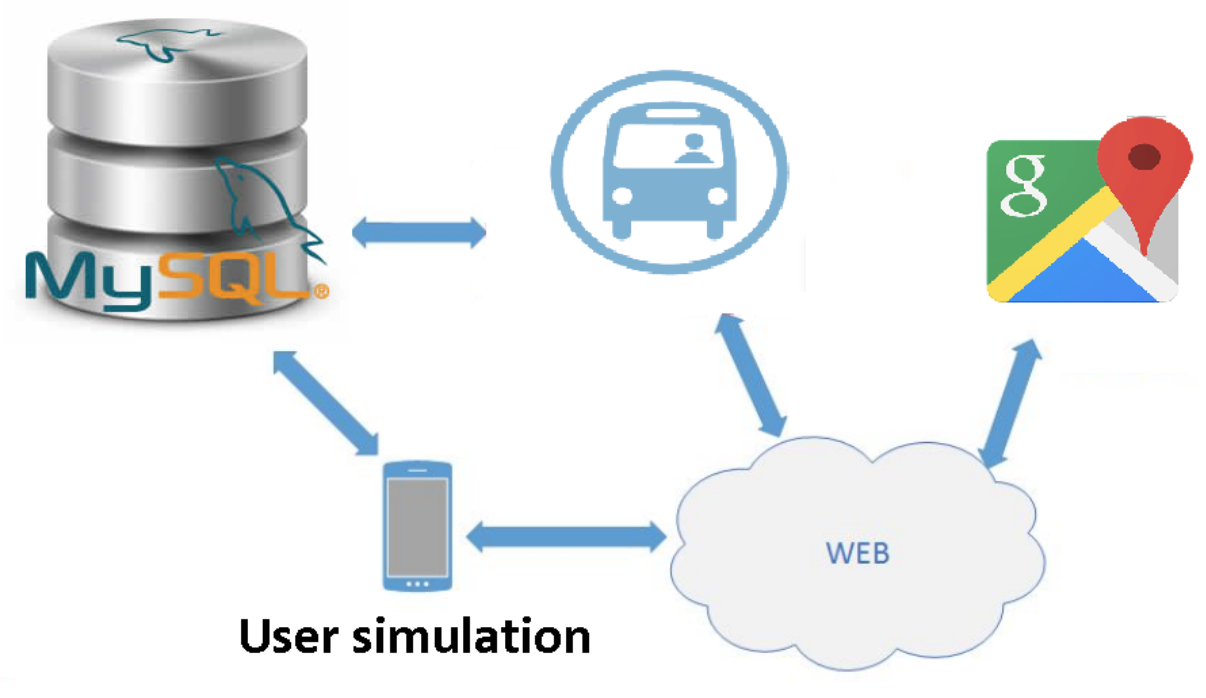
\includegraphics[width=14cm]{System_architecture}
\end{figure}
\subsection{Class diagram}
\begin{figure}[H]
	\centering
	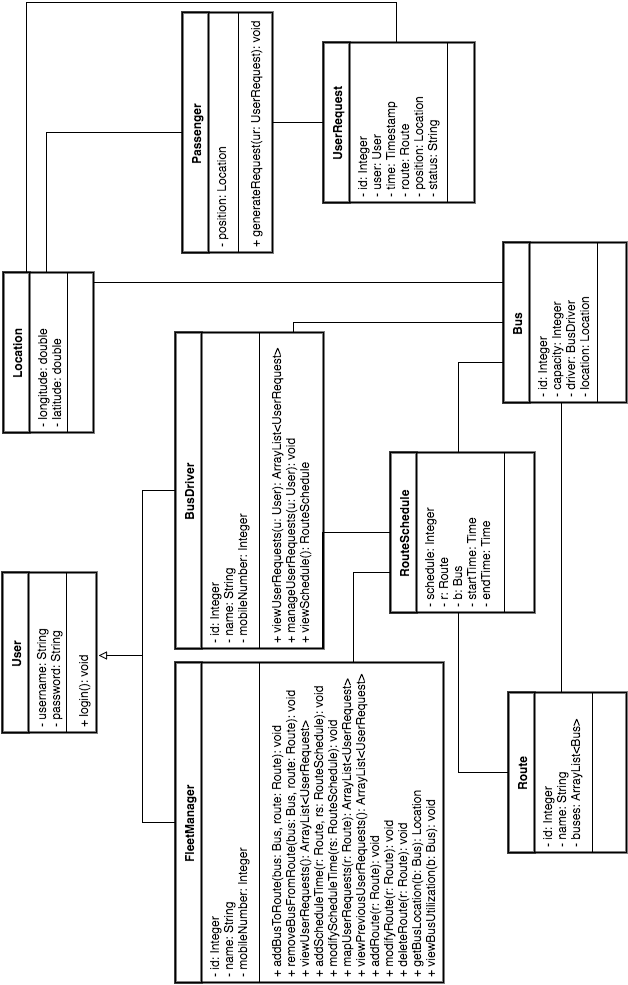
\includegraphics[height=19cm]{ClassDiagram}
\end{figure}